
% Default to the notebook output style

    


% Inherit from the specified cell style.




    
\documentclass{article}

    
    
    \usepackage{graphicx} % Used to insert images
    \usepackage{adjustbox} % Used to constrain images to a maximum size 
    \usepackage{color} % Allow colors to be defined
    \usepackage{enumerate} % Needed for markdown enumerations to work
    \usepackage{geometry} % Used to adjust the document margins
    \usepackage{amsmath} % Equations
    \usepackage{amssymb} % Equations
    \usepackage{eurosym} % defines \euro
    \usepackage[mathletters]{ucs} % Extended unicode (utf-8) support
    \usepackage[utf8x]{inputenc} % Allow utf-8 characters in the tex document
    \usepackage{fancyvrb} % verbatim replacement that allows latex
    \usepackage{grffile} % extends the file name processing of package graphics 
                         % to support a larger range 
    % The hyperref package gives us a pdf with properly built
    % internal navigation ('pdf bookmarks' for the table of contents,
    % internal cross-reference links, web links for URLs, etc.)
    \usepackage{hyperref}
    \usepackage{longtable} % longtable support required by pandoc >1.10
    \usepackage{booktabs}  % table support for pandoc > 1.12.2
    \usepackage{indentfirst}
    \usepackage{amsmath}
    \usepackage{floatrow}
    
    
    \definecolor{orange}{cmyk}{0,0.4,0.8,0.2}
    \definecolor{darkorange}{rgb}{.71,0.21,0.01}
    \definecolor{darkgreen}{rgb}{.12,.54,.11}
    \definecolor{myteal}{rgb}{.26, .44, .56}
    \definecolor{gray}{gray}{0.45}
    \definecolor{lightgray}{gray}{.95}
    \definecolor{mediumgray}{gray}{.8}
    \definecolor{inputbackground}{rgb}{.95, .95, .85}
    \definecolor{outputbackground}{rgb}{.95, .95, .95}
    \definecolor{traceback}{rgb}{1, .95, .95}
    % ansi colors
    \definecolor{red}{rgb}{.6,0,0}
    \definecolor{green}{rgb}{0,.65,0}
    \definecolor{brown}{rgb}{0.6,0.6,0}
    \definecolor{blue}{rgb}{0,.145,.698}
    \definecolor{purple}{rgb}{.698,.145,.698}
    \definecolor{cyan}{rgb}{0,.698,.698}
    \definecolor{lightgray}{gray}{0.5}
    
    % bright ansi colors
    \definecolor{darkgray}{gray}{0.25}
    \definecolor{lightred}{rgb}{1.0,0.39,0.28}
    \definecolor{lightgreen}{rgb}{0.48,0.99,0.0}
    \definecolor{lightblue}{rgb}{0.53,0.81,0.92}
    \definecolor{lightpurple}{rgb}{0.87,0.63,0.87}
    \definecolor{lightcyan}{rgb}{0.5,1.0,0.83}
    
    % commands and environments needed by pandoc snippets
    % extracted from the output of `pandoc -s`
    \providecommand{\tightlist}{%
      \setlength{\itemsep}{0pt}\setlength{\parskip}{0pt}}
    \DefineVerbatimEnvironment{Highlighting}{Verbatim}{commandchars=\\\{\}}
    % Add ',fontsize=\small' for more characters per line
    \newenvironment{Shaded}{}{}
    \newcommand{\KeywordTok}[1]{\textcolor[rgb]{0.00,0.44,0.13}{\textbf{{#1}}}}
    \newcommand{\DataTypeTok}[1]{\textcolor[rgb]{0.56,0.13,0.00}{{#1}}}
    \newcommand{\DecValTok}[1]{\textcolor[rgb]{0.25,0.63,0.44}{{#1}}}
    \newcommand{\BaseNTok}[1]{\textcolor[rgb]{0.25,0.63,0.44}{{#1}}}
    \newcommand{\FloatTok}[1]{\textcolor[rgb]{0.25,0.63,0.44}{{#1}}}
    \newcommand{\CharTok}[1]{\textcolor[rgb]{0.25,0.44,0.63}{{#1}}}
    \newcommand{\StringTok}[1]{\textcolor[rgb]{0.25,0.44,0.63}{{#1}}}
    \newcommand{\CommentTok}[1]{\textcolor[rgb]{0.38,0.63,0.69}{\textit{{#1}}}}
    \newcommand{\OtherTok}[1]{\textcolor[rgb]{0.00,0.44,0.13}{{#1}}}
    \newcommand{\AlertTok}[1]{\textcolor[rgb]{1.00,0.00,0.00}{\textbf{{#1}}}}
    \newcommand{\FunctionTok}[1]{\textcolor[rgb]{0.02,0.16,0.49}{{#1}}}
    \newcommand{\RegionMarkerTok}[1]{{#1}}
    \newcommand{\ErrorTok}[1]{\textcolor[rgb]{1.00,0.00,0.00}{\textbf{{#1}}}}
    \newcommand{\NormalTok}[1]{{#1}}
    
    % Define a nice break command that doesn't care if a line doesn't already
    % exist.
    \def\br{\hspace*{\fill} \\* }
    % Math Jax compatability definitions
    \def\gt{>}
    \def\lt{<}
    % Document parameters
    \title{Homework 11}
    \author{Roly Vicar\'ia \\ STAT501 Fall 2015}    
    
    

    % Pygments definitions
    
\makeatletter
\def\PY@reset{\let\PY@it=\relax \let\PY@bf=\relax%
    \let\PY@ul=\relax \let\PY@tc=\relax%
    \let\PY@bc=\relax \let\PY@ff=\relax}
\def\PY@tok#1{\csname PY@tok@#1\endcsname}
\def\PY@toks#1+{\ifx\relax#1\empty\else%
    \PY@tok{#1}\expandafter\PY@toks\fi}
\def\PY@do#1{\PY@bc{\PY@tc{\PY@ul{%
    \PY@it{\PY@bf{\PY@ff{#1}}}}}}}
\def\PY#1#2{\PY@reset\PY@toks#1+\relax+\PY@do{#2}}

\expandafter\def\csname PY@tok@gd\endcsname{\def\PY@tc##1{\textcolor[rgb]{0.63,0.00,0.00}{##1}}}
\expandafter\def\csname PY@tok@gu\endcsname{\let\PY@bf=\textbf\def\PY@tc##1{\textcolor[rgb]{0.50,0.00,0.50}{##1}}}
\expandafter\def\csname PY@tok@gt\endcsname{\def\PY@tc##1{\textcolor[rgb]{0.00,0.27,0.87}{##1}}}
\expandafter\def\csname PY@tok@gs\endcsname{\let\PY@bf=\textbf}
\expandafter\def\csname PY@tok@gr\endcsname{\def\PY@tc##1{\textcolor[rgb]{1.00,0.00,0.00}{##1}}}
\expandafter\def\csname PY@tok@cm\endcsname{\let\PY@it=\textit\def\PY@tc##1{\textcolor[rgb]{0.25,0.50,0.50}{##1}}}
\expandafter\def\csname PY@tok@vg\endcsname{\def\PY@tc##1{\textcolor[rgb]{0.10,0.09,0.49}{##1}}}
\expandafter\def\csname PY@tok@m\endcsname{\def\PY@tc##1{\textcolor[rgb]{0.40,0.40,0.40}{##1}}}
\expandafter\def\csname PY@tok@mh\endcsname{\def\PY@tc##1{\textcolor[rgb]{0.40,0.40,0.40}{##1}}}
\expandafter\def\csname PY@tok@go\endcsname{\def\PY@tc##1{\textcolor[rgb]{0.53,0.53,0.53}{##1}}}
\expandafter\def\csname PY@tok@ge\endcsname{\let\PY@it=\textit}
\expandafter\def\csname PY@tok@vc\endcsname{\def\PY@tc##1{\textcolor[rgb]{0.10,0.09,0.49}{##1}}}
\expandafter\def\csname PY@tok@il\endcsname{\def\PY@tc##1{\textcolor[rgb]{0.40,0.40,0.40}{##1}}}
\expandafter\def\csname PY@tok@cs\endcsname{\let\PY@it=\textit\def\PY@tc##1{\textcolor[rgb]{0.25,0.50,0.50}{##1}}}
\expandafter\def\csname PY@tok@cp\endcsname{\def\PY@tc##1{\textcolor[rgb]{0.74,0.48,0.00}{##1}}}
\expandafter\def\csname PY@tok@gi\endcsname{\def\PY@tc##1{\textcolor[rgb]{0.00,0.63,0.00}{##1}}}
\expandafter\def\csname PY@tok@gh\endcsname{\let\PY@bf=\textbf\def\PY@tc##1{\textcolor[rgb]{0.00,0.00,0.50}{##1}}}
\expandafter\def\csname PY@tok@ni\endcsname{\let\PY@bf=\textbf\def\PY@tc##1{\textcolor[rgb]{0.60,0.60,0.60}{##1}}}
\expandafter\def\csname PY@tok@nl\endcsname{\def\PY@tc##1{\textcolor[rgb]{0.63,0.63,0.00}{##1}}}
\expandafter\def\csname PY@tok@nn\endcsname{\let\PY@bf=\textbf\def\PY@tc##1{\textcolor[rgb]{0.00,0.00,1.00}{##1}}}
\expandafter\def\csname PY@tok@no\endcsname{\def\PY@tc##1{\textcolor[rgb]{0.53,0.00,0.00}{##1}}}
\expandafter\def\csname PY@tok@na\endcsname{\def\PY@tc##1{\textcolor[rgb]{0.49,0.56,0.16}{##1}}}
\expandafter\def\csname PY@tok@nb\endcsname{\def\PY@tc##1{\textcolor[rgb]{0.00,0.50,0.00}{##1}}}
\expandafter\def\csname PY@tok@nc\endcsname{\let\PY@bf=\textbf\def\PY@tc##1{\textcolor[rgb]{0.00,0.00,1.00}{##1}}}
\expandafter\def\csname PY@tok@nd\endcsname{\def\PY@tc##1{\textcolor[rgb]{0.67,0.13,1.00}{##1}}}
\expandafter\def\csname PY@tok@ne\endcsname{\let\PY@bf=\textbf\def\PY@tc##1{\textcolor[rgb]{0.82,0.25,0.23}{##1}}}
\expandafter\def\csname PY@tok@nf\endcsname{\def\PY@tc##1{\textcolor[rgb]{0.00,0.00,1.00}{##1}}}
\expandafter\def\csname PY@tok@si\endcsname{\let\PY@bf=\textbf\def\PY@tc##1{\textcolor[rgb]{0.73,0.40,0.53}{##1}}}
\expandafter\def\csname PY@tok@s2\endcsname{\def\PY@tc##1{\textcolor[rgb]{0.73,0.13,0.13}{##1}}}
\expandafter\def\csname PY@tok@vi\endcsname{\def\PY@tc##1{\textcolor[rgb]{0.10,0.09,0.49}{##1}}}
\expandafter\def\csname PY@tok@nt\endcsname{\let\PY@bf=\textbf\def\PY@tc##1{\textcolor[rgb]{0.00,0.50,0.00}{##1}}}
\expandafter\def\csname PY@tok@nv\endcsname{\def\PY@tc##1{\textcolor[rgb]{0.10,0.09,0.49}{##1}}}
\expandafter\def\csname PY@tok@s1\endcsname{\def\PY@tc##1{\textcolor[rgb]{0.73,0.13,0.13}{##1}}}
\expandafter\def\csname PY@tok@kd\endcsname{\let\PY@bf=\textbf\def\PY@tc##1{\textcolor[rgb]{0.00,0.50,0.00}{##1}}}
\expandafter\def\csname PY@tok@sh\endcsname{\def\PY@tc##1{\textcolor[rgb]{0.73,0.13,0.13}{##1}}}
\expandafter\def\csname PY@tok@sc\endcsname{\def\PY@tc##1{\textcolor[rgb]{0.73,0.13,0.13}{##1}}}
\expandafter\def\csname PY@tok@sx\endcsname{\def\PY@tc##1{\textcolor[rgb]{0.00,0.50,0.00}{##1}}}
\expandafter\def\csname PY@tok@bp\endcsname{\def\PY@tc##1{\textcolor[rgb]{0.00,0.50,0.00}{##1}}}
\expandafter\def\csname PY@tok@c1\endcsname{\let\PY@it=\textit\def\PY@tc##1{\textcolor[rgb]{0.25,0.50,0.50}{##1}}}
\expandafter\def\csname PY@tok@kc\endcsname{\let\PY@bf=\textbf\def\PY@tc##1{\textcolor[rgb]{0.00,0.50,0.00}{##1}}}
\expandafter\def\csname PY@tok@c\endcsname{\let\PY@it=\textit\def\PY@tc##1{\textcolor[rgb]{0.25,0.50,0.50}{##1}}}
\expandafter\def\csname PY@tok@mf\endcsname{\def\PY@tc##1{\textcolor[rgb]{0.40,0.40,0.40}{##1}}}
\expandafter\def\csname PY@tok@err\endcsname{\def\PY@bc##1{\setlength{\fboxsep}{0pt}\fcolorbox[rgb]{1.00,0.00,0.00}{1,1,1}{\strut ##1}}}
\expandafter\def\csname PY@tok@mb\endcsname{\def\PY@tc##1{\textcolor[rgb]{0.40,0.40,0.40}{##1}}}
\expandafter\def\csname PY@tok@ss\endcsname{\def\PY@tc##1{\textcolor[rgb]{0.10,0.09,0.49}{##1}}}
\expandafter\def\csname PY@tok@sr\endcsname{\def\PY@tc##1{\textcolor[rgb]{0.73,0.40,0.53}{##1}}}
\expandafter\def\csname PY@tok@mo\endcsname{\def\PY@tc##1{\textcolor[rgb]{0.40,0.40,0.40}{##1}}}
\expandafter\def\csname PY@tok@kn\endcsname{\let\PY@bf=\textbf\def\PY@tc##1{\textcolor[rgb]{0.00,0.50,0.00}{##1}}}
\expandafter\def\csname PY@tok@mi\endcsname{\def\PY@tc##1{\textcolor[rgb]{0.40,0.40,0.40}{##1}}}
\expandafter\def\csname PY@tok@gp\endcsname{\let\PY@bf=\textbf\def\PY@tc##1{\textcolor[rgb]{0.00,0.00,0.50}{##1}}}
\expandafter\def\csname PY@tok@o\endcsname{\def\PY@tc##1{\textcolor[rgb]{0.40,0.40,0.40}{##1}}}
\expandafter\def\csname PY@tok@kr\endcsname{\let\PY@bf=\textbf\def\PY@tc##1{\textcolor[rgb]{0.00,0.50,0.00}{##1}}}
\expandafter\def\csname PY@tok@s\endcsname{\def\PY@tc##1{\textcolor[rgb]{0.73,0.13,0.13}{##1}}}
\expandafter\def\csname PY@tok@kp\endcsname{\def\PY@tc##1{\textcolor[rgb]{0.00,0.50,0.00}{##1}}}
\expandafter\def\csname PY@tok@w\endcsname{\def\PY@tc##1{\textcolor[rgb]{0.73,0.73,0.73}{##1}}}
\expandafter\def\csname PY@tok@kt\endcsname{\def\PY@tc##1{\textcolor[rgb]{0.69,0.00,0.25}{##1}}}
\expandafter\def\csname PY@tok@ow\endcsname{\let\PY@bf=\textbf\def\PY@tc##1{\textcolor[rgb]{0.67,0.13,1.00}{##1}}}
\expandafter\def\csname PY@tok@sb\endcsname{\def\PY@tc##1{\textcolor[rgb]{0.73,0.13,0.13}{##1}}}
\expandafter\def\csname PY@tok@k\endcsname{\let\PY@bf=\textbf\def\PY@tc##1{\textcolor[rgb]{0.00,0.50,0.00}{##1}}}
\expandafter\def\csname PY@tok@se\endcsname{\let\PY@bf=\textbf\def\PY@tc##1{\textcolor[rgb]{0.73,0.40,0.13}{##1}}}
\expandafter\def\csname PY@tok@sd\endcsname{\let\PY@it=\textit\def\PY@tc##1{\textcolor[rgb]{0.73,0.13,0.13}{##1}}}

\def\PYZbs{\char`\\}
\def\PYZus{\char`\_}
\def\PYZob{\char`\{}
\def\PYZcb{\char`\}}
\def\PYZca{\char`\^}
\def\PYZam{\char`\&}
\def\PYZlt{\char`\<}
\def\PYZgt{\char`\>}
\def\PYZsh{\char`\#}
\def\PYZpc{\char`\%}
\def\PYZdl{\char`\$}
\def\PYZhy{\char`\-}
\def\PYZsq{\char`\'}
\def\PYZdq{\char`\"}
\def\PYZti{\char`\~}
% for compatibility with earlier versions
\def\PYZat{@}
\def\PYZlb{[}
\def\PYZrb{]}
\makeatother


    % Exact colors from NB
    \definecolor{incolor}{rgb}{0.0, 0.0, 0.5}
    \definecolor{outcolor}{rgb}{0.545, 0.0, 0.0}



    
    % Prevent overflowing lines due to hard-to-break entities
    \sloppy 
    % Setup hyperref package
    \hypersetup{
      breaklinks=true,  % so long urls are correctly broken across lines
      colorlinks=true,
      urlcolor=blue,
      linkcolor=darkorange,
      citecolor=darkgreen,
      }
    % Slightly bigger margins than the latex defaults
    
    \geometry{verbose,tmargin=1in,bmargin=1in,lmargin=.5in,rmargin=.5in}
    
    

    \begin{document}
    
    
    \maketitle
    
    

    
    \subsubsection{Question 1}\label{question-1}

    \begin{center}
Results of Regression Analyses
\end{center}

\begin{longtable}[c]{@{}lllllp{6cm}ll@{}}
\toprule
Part & Model & L & N & E & Sample equation
& S & \(R^2\) adj\tabularnewline
\midrule
\endhead
b & savings vs age & N & Y & Y & savings = 1.92 + 1.5247 age & 3.56198 &
99.76\%\tabularnewline
c & savings vs age, income & N & Y & Y & savings = -11.27 +~0.830~age
+~0.952~income & 3.46443 & 91.26\%\tabularnewline
f & savingsnew vs agenew, incomenew & N & Y & N & savingsnew = -14.53
+~0.6757~agenew +~1.177~incomenew & 3.50033 & 90.27\%\tabularnewline
h & savingsnew vs agenew, incomenew, \(agenew^2\) & Y & Y & N &
savingsnew = 3.49 -~0.441~agenew +~1.179~incomenew
+~0.01636~agenew*agenew & 3.40931 & 90.77\%\tabularnewline
j & savingsnew vs agenewc, incomenew, \(agenewc^2\) & Y & Y & N &
savingsnew = 7.22 +~0.6624~agenewc +~1.179~incomenew
+~0.01636~agenewc*agenewc & 3.40931 & 90.77\%\tabularnewline
\bottomrule
\end{longtable}

\begin{enumerate}
\def\labelenumi{\alph{enumi})}
\tightlist
\item
  The matrix plot shows that savings has a strong correlation with age
  and a strong correlation with income. It also shows that age has a
  strong correlation with income. It suggests that an MLR model with
  both predictors will have larger standard error for the estimated
  coefficients and marginal (if any) contribution to reducing the error
  sum of squares from the second predictor.
  
  \begin{figure}[h!]
 \centering
 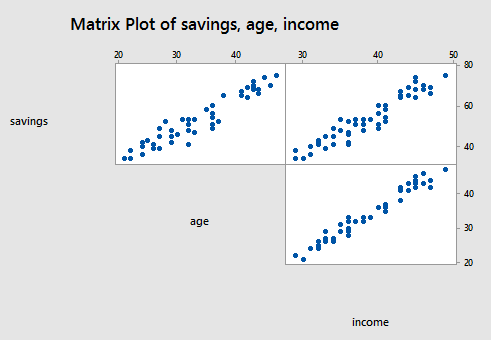
\includegraphics[scale=.5]{./images/matrix-plot_savings-age-income.png}
 % matrix-plot_savings-age-income.png: 491x340 pixel, 96dpi, 12.99x8.99 cm, bb=0 0 368 255
\end{figure}

\end{enumerate}

\newpage
\begin{enumerate}
\def\labelenumi{\alph{enumi})}
\setcounter{enumi}{1}
\tightlist
\item
  The residuals vs fits plot for this model look good. The visual
  inspection suggests equal variances. The lack of linearity isn't
  obvious, but there is a subtle up-down-up pattern in the data. The
  normality test for the residuals confirms that they are normally
  distributed.
  
  \begin{figure}[!h]
  \begin{floatrow}
   \ffigbox{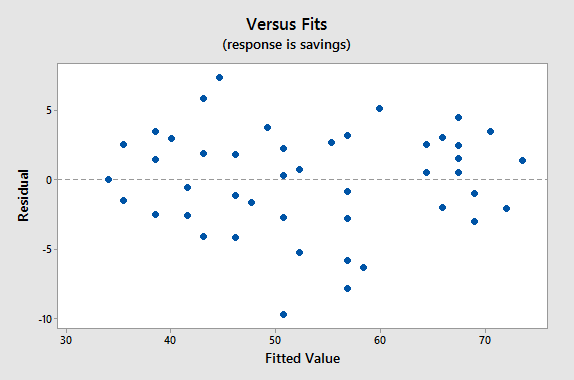
\includegraphics[scale=0.5]{./images/plot-residuals-vs-fits_savings-vs-age.png}}{}
   \ffigbox{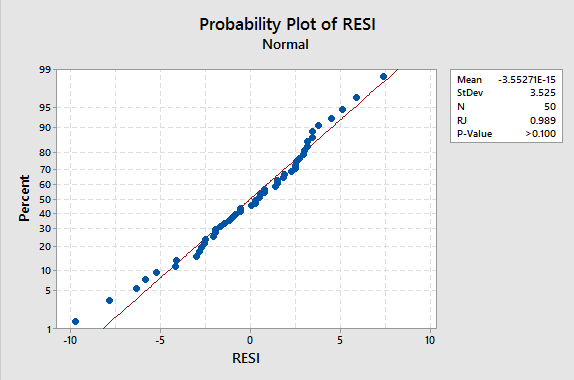
\includegraphics[scale=0.5]{./images/probability-plot_normality-of-residuals_savings-vs-age.png}}{}
  \end{floatrow}
\end{figure}
  
\end{enumerate}

\begin{enumerate}
\def\labelenumi{\alph{enumi})}
\setcounter{enumi}{2}
\tightlist
\item
  The residuals vs fits plot shows that the up-down-up pattern from the
  previous model is actually accentuated by adding the income predictor
  to the model. The variances appear equal, however. And the normality
  test confirms that they are normally distributed.
  
\begin{figure}[!h]
  \begin{floatrow}
   \ffigbox{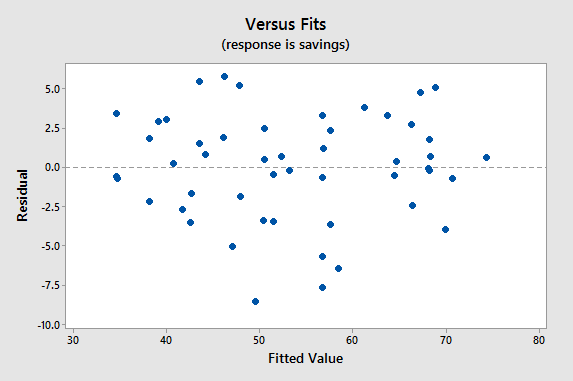
\includegraphics[scale=0.5]{./images/plot-residuals-vs-fits_savings-vs-age-and-income.png}}{}
   \ffigbox{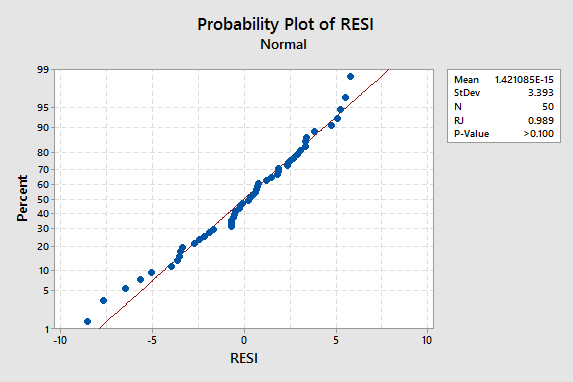
\includegraphics[scale=0.5]{./images/probability-plot_normality-of-residuals_savings-vs-age-and-income.png}}{}
  \end{floatrow}
\end{figure}
\end{enumerate}

\begin{enumerate}
\def\labelenumi{\alph{enumi})}
\setcounter{enumi}{3}
\item
  From the model in part (c), age and income both had the same VIF value
  of 29.29. This indicates a high level of correlation between the two
  predictors. This suggests that the MLR model that includes these two
  predictors would have less precision of the estimated regression
  coefficients. The estimated coefficients will be dependent on each
  other and have different values than from independent SLR models. We
  can mitigate these problems by removing one of the predictors from the
  model.
  
\newpage
\item
  Comparing this matrix plot with that from part (a), it looks like
  agenew and incomenew are highly correlated, but slightly less so than
  the age and income from part (a).
  
\begin{figure}[h!]
 \centering
 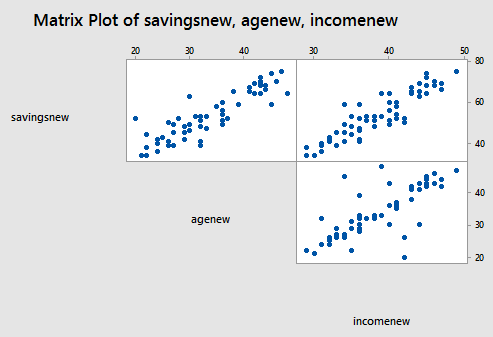
\includegraphics[scale=.5]{./images/matrix-plot_savingsnew-agenew-incomenew.png}
 % matrix-plot_savingsnew-agenew-incomenew.png: 493x337 pixel, 96dpi, 13.04x8.92 cm, bb=0 0 370 253
\end{figure}

\end{enumerate}

\begin{enumerate}
\def\labelenumi{\alph{enumi})}
\setcounter{enumi}{5}
\tightlist
\item
  The residuals vs fits plot still shows the up-down-up pattern from
  previous plots. It looks however, that now the variance is no longer
  equal. It seems less at the ends and greater in the center.
  
\begin{figure}[!h]
  \begin{floatrow}
   \ffigbox{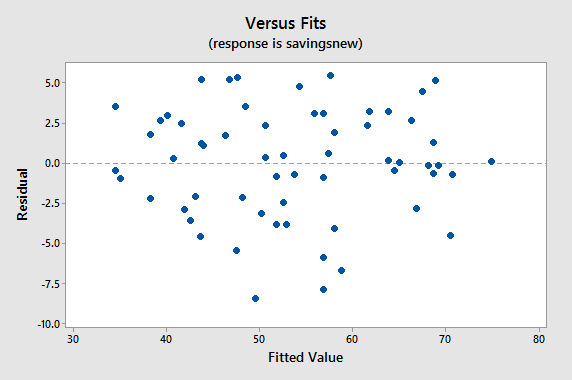
\includegraphics[scale=0.5]{./images/plot-residuals-vs-fits_savingsnew-vs-agenew-and-incomenew.png}}{}
   \ffigbox{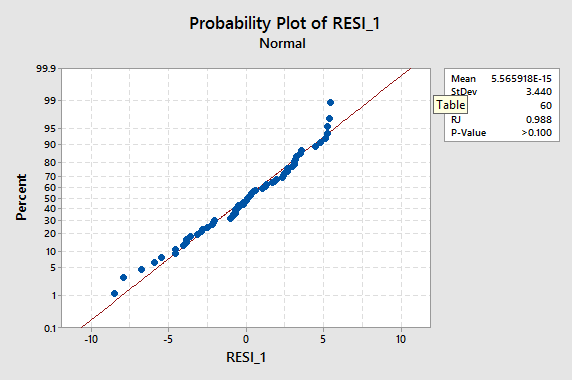
\includegraphics[scale=0.5]{./images/probability-plot_normality-of-residuals_savingsnew-vs-agenew-and-incomenew.png}}{}
  \end{floatrow}
\end{figure}
\end{enumerate}

\begin{enumerate}
\def\labelenumi{\alph{enumi})}
\setcounter{enumi}{6}
\item
  From the model in part (f), agenew and incomenew both have the same
  VIF value of 2.48. This indicates a slight level of correlation
  between the two predictors, but nothing that would warrant further
  investigation according to the rule of thumb given in the notes. It
  appears as though the regression pitfalls have been mitigated.
\item
  I believe that the model generated by adding the \(agenew^2\) term has
  addressed the linearity issues of the previous models, but it still
  seems to have non-equal variances, larger in the center and smaller at
  the ends. The probability plot confirms that the errors are normally
  distributed.
  
\begin{figure}[!h]
  \begin{floatrow}
   \ffigbox{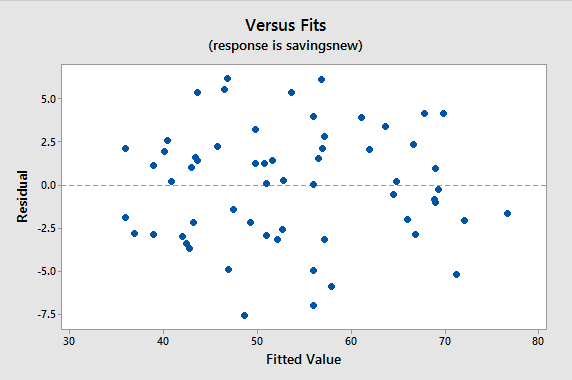
\includegraphics[scale=0.5]{./images/plot-residuals-vs-fits_savingsnew-vs-agenew-incomenew-agenew2.png}}{}
   \ffigbox{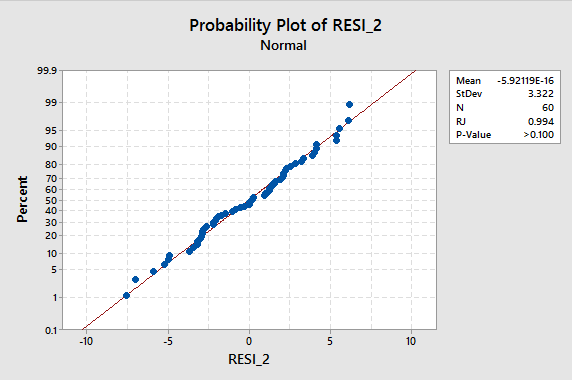
\includegraphics[scale=0.5]{./images/probability-plot_normality-of-residuals_savingsnew-vs-agenew-incomenew-agenew2.png}}{}
  \end{floatrow}
\end{figure}
  
\end{enumerate}

\begin{enumerate}
\def\labelenumi{\roman{enumi})}
\tightlist
\item
  The VIFs in the previous part are 94.15 for agenew and 92.51 for
  \(agenew^2\). This indicates a strong correlation between these
  predictors that could affect the precision of the estimated
  coefficients, as well as causing the estimated coefficients to be
  dependent on each other. We can remove one of the predictors to
  mitigate this.
\end{enumerate}

\begin{enumerate}
\def\labelenumi{\alph{enumi})}
\setcounter{enumi}{9}
\tightlist
\item
  The residuals vs fits plot of this model looks identical to that from
  part (h). The regression equation has changed slightly since the
  agenewc column has a different range of values.
  
\begin{figure}[!h]
  \begin{floatrow}
   \ffigbox{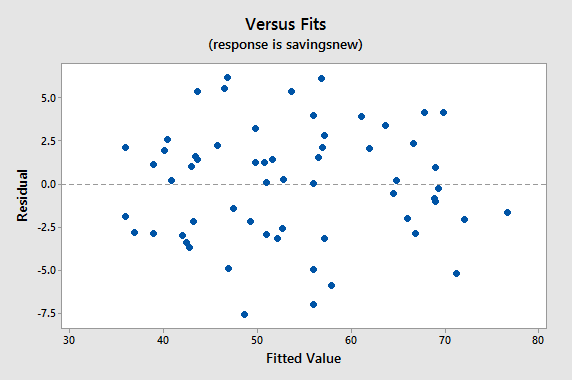
\includegraphics[scale=0.5]{./images/plot-residuals-vs-fits_savingsnew-vs-agenewc-incomenew-agenewc2.png}}{}
   \ffigbox{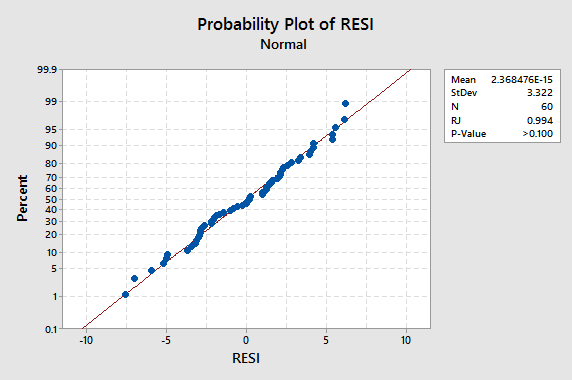
\includegraphics[scale=0.5]{./images/probability-plot_normality-of-residuals_savingsnew-vs-agenewc-incomenew-agenewc2.png}}{}
  \end{floatrow}
\end{figure}
\end{enumerate}

\begin{enumerate}
\def\labelenumi{\alph{enumi})}
\setcounter{enumi}{10}
\item
  The VIFs for agenewc and \(agenewc^2\) are 2.5 and 1.01, respectively.
  It would appear that the pitfalls from part (i) have been mitigated.
\item
  The prediction of savingsnew for an individual with agenew = 30 and
  incomenew = 45, using the model from part (h), is 58.0455. Using the
  model from part (j), is 58.0455. Both models arrive at the exact same
  prediction which makes sense since we saw that multicollinearity
  doesn't have a huge impact on predictions especially for values close
  to the means of the predictors.
\end{enumerate}

    \subsubsection{Question 2}\label{question-2}

\begin{enumerate}
\def\labelenumi{\alph{enumi})}
\item
\end{enumerate}

\begin{longtable}[c]{@{}lllll@{}}
\toprule
Model & \(b_1\) & \(se(b_1)\) & \(b_2\) & \(se(b_2)\)\tabularnewline
\midrule
\endhead
savings vs age & 1.5247 & 0.0694 ~ & XXX & XXX\tabularnewline
savings vs income & XXX & XXX & 2.0493 & 0.0948 ~\tabularnewline
savings vs age, income & 0.830 & 0.366 & 0.952 & 0.492\tabularnewline
savingsnew vs agenew & 1.2930 & 0.0887 & XXX & XXX\tabularnewline
savingsnew vs incomenew & XXX & XXX & 1.947 & 0.120\tabularnewline
savingsnew vs agenew, incomenew & 0.6757 & 0.0934 & 1.177 &
0.138\tabularnewline
\bottomrule
\end{longtable}

\begin{enumerate}
\def\labelenumi{\alph{enumi})}
\setcounter{enumi}{1}
\item
  \begin{enumerate}
  \def\labelenumii{\roman{enumii}.}
  \tightlist
  \item
    We can see that in the first 3 models, the estimated coefficients
    vary significantly from the SLR models to the MLR model. The age
    coefficient went from 1.5247 in the SLR to 0.830 in the MLR. Same
    thing from income: from 2.0493 to 0.952. Both reduced by about half.
  \item
    We see that the standard error for both predictors increases by a
    little over 500\% from the SLRs to the MLR.
  \end{enumerate}
\item
  \begin{enumerate}
  \def\labelenumii{\roman{enumii}.}
  \tightlist
  \item
    The estimated coefficient of agenew shows that it's still dependent
    on incomenew since it drops by about 50\% from one model to the
    other. The incomenew coefficient shows better invariance across
    models, but still drops considerably.
  \item
    The standard errors of the estimated coefficients do remain
    approximately the same from the SLRs to the MLR.
  \end{enumerate}
\end{enumerate}

\newpage
    \subsubsection{Question 3}\label{question-3}

\begin{enumerate}
\def\labelenumi{\alph{enumi})}
\tightlist
\item
  The plot of StopDist vs spdmn19 shows a strong positive correlation
  between the variables. The relationship appears to be non-linear since
  it's curving upwards. The variance in StopDist also seems to increase
  as spdmn19 increases.
  
\begin{figure}[h!]
 \centering
 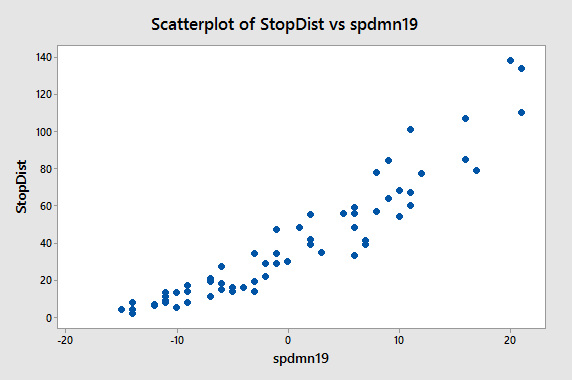
\includegraphics[scale=.5]{./images/scatterplot_StopDist-vs-spdmn19.png}
 % scatterplot_StopDist-vs-spdmn19.png: 572x380 pixel, 96dpi, 15.13x10.05 cm, bb=0 0 429 285
\end{figure}

\end{enumerate}

\begin{enumerate}
\def\labelenumi{\alph{enumi})}
\setcounter{enumi}{1}
\tightlist
\item
  \(StopDist = 32.91 + 2.902 spdmn19 + 0.0666 spdsqrd\)
  
  \begin{figure}[h!]
 \centering
 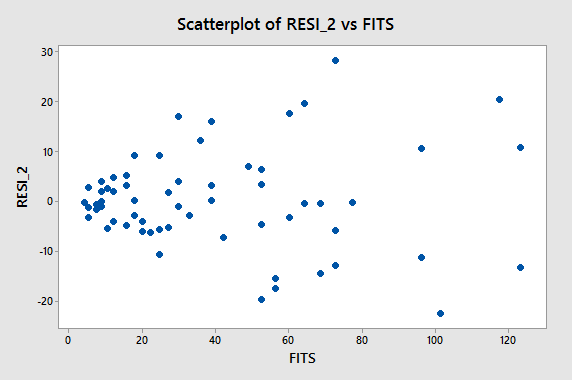
\includegraphics[scale=.5]{./images/plot-residuals-vs-fits_stopDist-vs-spdmn19-and-spdsqrd.png}
 % plot-residuals-vs-fits_stopDist-vs-spdmn19-and-spdsqrd.png: 572x380 pixel, 96dpi, 15.13x10.05 cm, bb=0 0 429 285
\end{figure}

\end{enumerate}

The residual plot indicates that the variance is not constant. It
increases for larger fitted values. Also, there seems to be a larger
concentration of data points for smaller fitted values and grows more
sparse as we move to the right.

\begin{enumerate}
\def\labelenumi{\alph{enumi})}
\setcounter{enumi}{2}
\item
\end{enumerate}

\begin{longtable}[c]{@{}lll@{}}
\toprule
Coefficient & Coefficient Value & Standard Error\tabularnewline
\midrule
\endhead
\(b_0\) (constant) & 32.91 & 1.76\tabularnewline
\(b_1\) (linear term) & 2.902 & 0.135\tabularnewline
\(b_2\) (quadratic term) & 0.0666 & 0.0129\tabularnewline
\bottomrule
\end{longtable}

\begin{enumerate}
\def\labelenumi{\alph{enumi})}
\setcounter{enumi}{3}
\item
\end{enumerate}

\begin{longtable}[c]{@{}lll@{}}
\toprule
Coefficient & Coefficient Value & Standard Error\tabularnewline
\midrule
\endhead
\(b_0\) (constant) & 33.08 & 1.35\tabularnewline
\(b_1\) (linear term) & 2.908 & 0.132\tabularnewline
\(b_2\) (quadratic term) & 0.0650 & 0.0122\tabularnewline
\bottomrule
\end{longtable}

\begin{enumerate}
\def\labelenumi{\alph{enumi})}
\setcounter{enumi}{4}
\item
  The results are almost the same for both models. The coefficient
  values and standard errors varied only slightly. The largest change
  was the standard error for the constant term which changed from 1.76
  to 1.35.
\item
  The plot of studentized residuals vs fits looks much better than the
  previous plot in terms of correcting the error variance. This plot
  appears much closer to a horizontal band with constant variance. There
  does still appear to be a denser concentration of data points for
  smaller fitted values, and gets sparser for larger fitted values.
  
  \begin{figure}[h!]
 \centering
 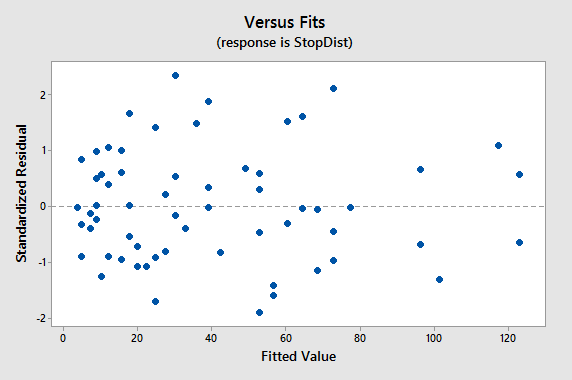
\includegraphics[scale=0.5]{./images/plot-standardized-residuals-vs-fits_stopDist-vs-spdmn19-and-spdsqrd.png}
 % plot-standardized-residuals-vs-fits_stopDist-vs-spdmn19-and-spdsqrd.png: 572x380 pixel, 96dpi, 15.13x10.05 cm, bb=0 0 429 285
\end{figure}

\end{enumerate}


    % Add a bibliography block to the postdoc
    
    
    
    \end{document}
